\documentclass[preview,tikz]{standalone}

\usepackage{amsmath}
\usepackage{upgreek}
\usepackage{xcolor}
\usepackage[sc]{mathpazo}
\linespread{1.05}
\usepackage[T1]{fontenc}

\definecolor{hudbg}{rgb}{0.2,0.2,0.2}
\definecolor{triadbg}{rgb}{0.15,0.15,0.15}
\definecolor{graphbg}{rgb}{0.15,0.15,0.15}
\definecolor{border}{rgb}{0.175,0.175,0.175}

% White theme
% \definecolor{hudbg}{rgb}{0.8,0.8,0.8}
% \definecolor{triadbg}{rgb}{0.65,0.65,0.65}
% \definecolor{graphbg}{rgb}{0.65,0.65,0.65}
% \definecolor{border}{rgb}{0.60,0.60,0.60}

\renewcommand{\vec}[1]{\mathbf{#1}}
\newcommand{\mat}[1]{\mathbf{#1}}

\tikzset{every picture/.style={line width=1pt}}

\begin{document}
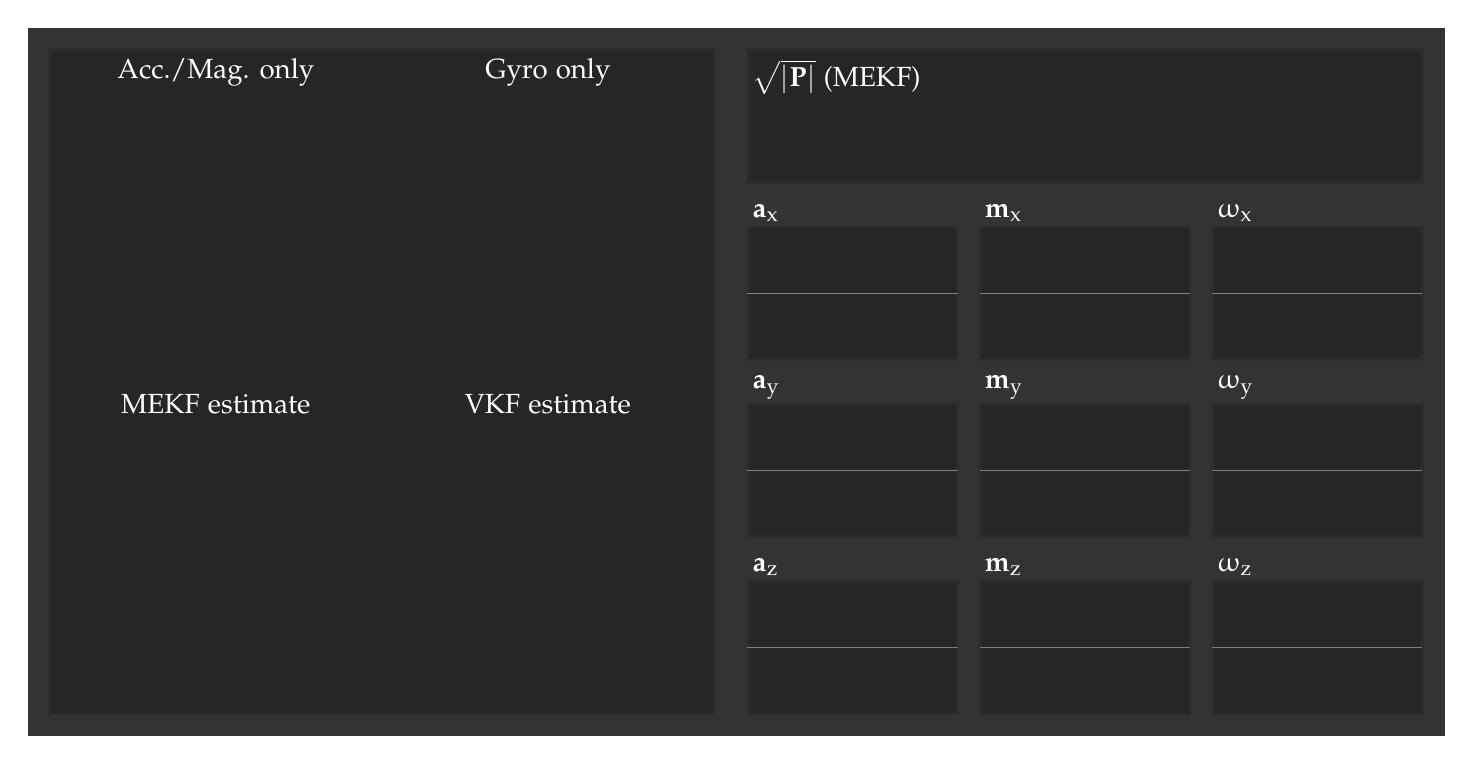
\begin{tikzpicture}[x=1pt,y=1pt,scale=0.4]

\fill[color=hudbg] (0,0) rectangle (1280,640);
\fill[color=triadbg] (20,20) rectangle (620,620);
\draw[color=border] (20,20) rectangle (620,620);

\node[color=white] at (170, 600) {Acc./Mag. only};
\node[color=white] at (470, 600) {Gyro only};
\node[color=white] at (170, 300) {MEKF estimate};
\node[color=white] at (470, 300) {VKF estimate};

\begin{scope}[xshift=640]
  \fill[color=graphbg] (10,500) rectangle (620,620);
  \node[color=white, above right] at (5,570) {$\sqrt{\left\lvert\vec{P}\right\rvert}$ (MEKF)};
  \draw[color=border] (10,500) rectangle (620,620);

  % \draw[color=gray, thin] (10,{80+160*(\i-1)}) -- (200,{80+160*(\i-1)});

  \foreach[count=\i] \k in {z, y, x}
  {
    \fill[color=graphbg] (10,{20+160*(\i-1)}) rectangle (200,{140+160*(\i-1)});
    \draw[color=border] (10,{20+160*(\i-1)}) rectangle (200,{140+160*(\i-1)});
    \node[color=white, above right] at (5,{135+160*(\i-1)}) {$\vec{a}_\mathrm{\k}$};
    \draw[color=gray, thin] (10,{80+160*(\i-1)}) -- (200,{80+160*(\i-1)});

    \fill[color=graphbg] (220,{20+160*(\i-1)}) rectangle (410,{140+160*(\i-1)});
    \draw[color=border] (220,{20+160*(\i-1)}) rectangle (410,{140+160*(\i-1)});
    \node[color=white, above right] at (215,{135+160*(\i-1)}) {$\vec{m}_\mathrm{\k}$};
    \draw[color=gray, thin] (220,{80+160*(\i-1)}) -- (410,{80+160*(\i-1)});

    \fill[color=graphbg] (430,{20+160*(\i-1)}) rectangle (620,{140+160*(\i-1)});
    \draw[color=border] (430,{20+160*(\i-1)}) rectangle (620,{140+160*(\i-1)});
    \node[color=white, above right] at (425,{135+160*(\i-1)}) {$\vec{\upomega}_\mathrm{\k}$};
    \draw[color=gray, thin] (430,{80+160*(\i-1)}) -- (620,{80+160*(\i-1)});
  }
\end{scope}

%\node[draw, circle, color=white] at (40pt,40pt) {$x$};

\end{tikzpicture}
\end{document}